\documentclass[12pt, a4paper]{article}

\usepackage[default]{sourcesanspro}
\usepackage[T1]{fontenc}
\usepackage[french]{babel}
\usepackage[autolanguage]{numprint}
\usepackage{hyperref}
\usepackage{graphicx}
\usepackage{array}
\usepackage{multirow}
\usepackage{colortbl}
\usepackage{tikz}
\hypersetup{
    colorlinks=true,
    linkcolor=black,
    urlcolor=red,
    pdftitle={NLP Lab3 Report},
}
\usepackage{geometry}
\geometry{left=0.5in, right=0.5in, top=0.5in, bottom=1in}
\usepackage{setspace}
\onehalfspacing
\usepackage[language=french]{lipsum}
\usepackage{mfirstuc}  % For capitalizing words
\usepackage{titlesec}   % For title formatting
\usepackage{ragged2e}
\usepackage{float}

\begin{document}
\begin{titlepage}

\newgeometry{left=0.5in, right=0.5in, top=0.5in, bottom=0.5in}


\begin{minipage}[t]{\linewidth}
\centering
\capitalisewords{République Algerienne Démocratique et Populaire} \\
\capitalisewords{Ministère de l'enseignement supérieur et de la recherche scientifique} \\
\capitalisewords{École supérieure en informatique 8 Mai 1945 Sidi Bel-Abbés} \\
\end{minipage}
\vspace{12pt}
\hrule


\vspace{4cm}

\begin{center}

\vspace{2.5cm}


\huge{\capitalisewords{NLP Lab 3 Report}}

\vspace{0.5cm}

\normalsize
\uppercase{\textbf{Benyamina Yacine Lazreg}}
\normalsize
\uppercase{\textbf{IASD - G01}}

\texttt{
\href{mailto:yl.benyamina@esi-sba.dz}{yl.benyamina@esi-sba.dz}
}

\today

\vspace{2.5cm}


\vfill

\large
2023 - 2024 \\
%\vspace{8pt}
%\hrule


\end{center}
\end{titlepage}


\thispagestyle{empty}
\clearpage

\section {Results from previous labs}

After exporting the cleaned and stemmed text which was realised in Lab 1 and training it using different techniques and models (Lab 2) the following results were obtained:

\begin{figure}[H]
    \centering
    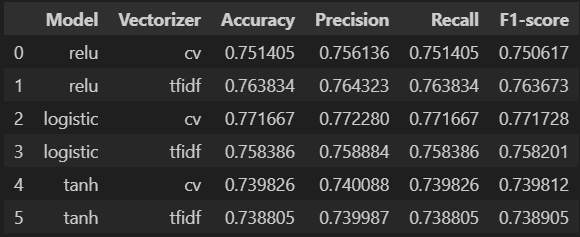
\includegraphics[width=0.5\linewidth]{df1.png}
    \caption{Results of using a combination of different activation functions and vectorizations methods}
    \label{fig:enter-label}
\end{figure}

\begin{figure}[H]
    \centering
    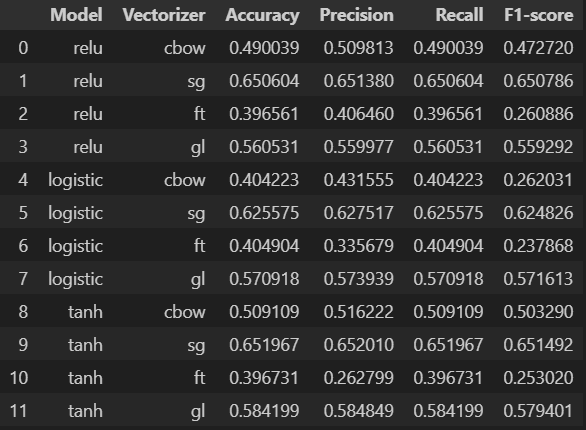
\includegraphics[width=0.5\linewidth]{df2.png}
    \caption{Results of using a combination of different activation functions and embedding methods}
    \label{fig:enter-label}
\end{figure}

According to the figures we can clearly see that the model which uses CountVectorizer and Sigmoid activation function has the best results across all metrics, this is going to be the model that we'll try to improve.

\begin{figure}[H]
    \centering
    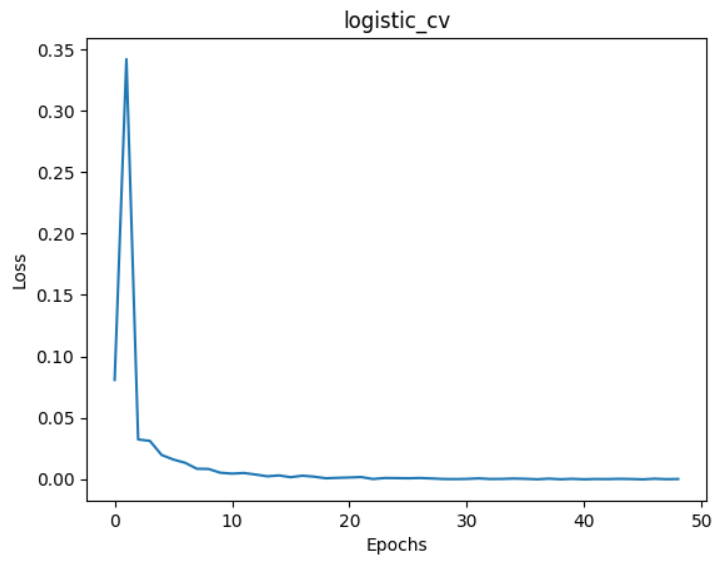
\includegraphics[width=0.5\linewidth]{cvloss.png}
    \caption{The loss graph of the best model}
    \label{fig:enter-label}
\end{figure}

\section{Improving the model}
The model was trained on a simple architecture of two hidden layers of size (32, 64) with Sigmoid activation function, a learning rate of 0.01 and Adam Optimizer. \newline \\
The trivial thing to do is to try Random Search to try and improve the architecture of the neural network, therefore Random Search was realized with 3 target variables; 
\begin{itemize}
    \item The number of neurons in the first layer which is a choice between [8, 16, 32, 64, 128] neurons
    \item The number of neurons in the second layer which is a choice between [8, 16, 32, 64, 128] neurons
    \item The learning rate which is a random value between 0.0001 and 0.01 and follows the log sampling  \\
\end{itemize}


It is also worth noting that adding Dropout as another variable with random value between 0.1 and 0.5 was tried but canceled later because after running more than 20 trials with dropout as a parameter the model could not achieve an accuracy higher than 40\% \\

Running the Random Search for 100 trials, with Adam optimizer and 10 epochs each yields the following results: 

\begin{figure}[H]
    \centering
    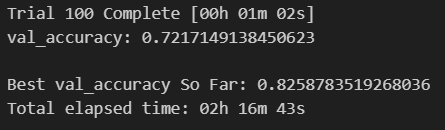
\includegraphics[width=0.5\linewidth]{search.png}
    \caption{Result of 100 trials}
    \label{fig:enter-label}
\end{figure}

\begin{figure}[H]
    \centering
    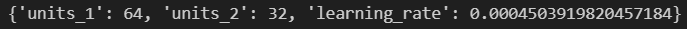
\includegraphics[width=0.5\linewidth]{hp.png}
    \caption{The best Hyper parameters}
    \label{fig:enter-label}
\end{figure}

The best obtained Hyper parameters were: 
\begin{itemize}
    \item 64 neurons for the first hidden layer
    \item 32 neurons for the second hidden layer
    \item A learning rate of 0.00045039 \\
\end{itemize}

\section{Final results and discussion}
After running the model with the best Hyper parameters for 15 epochs the following results were obtained:

\begin{figure}[H]
    \centering
    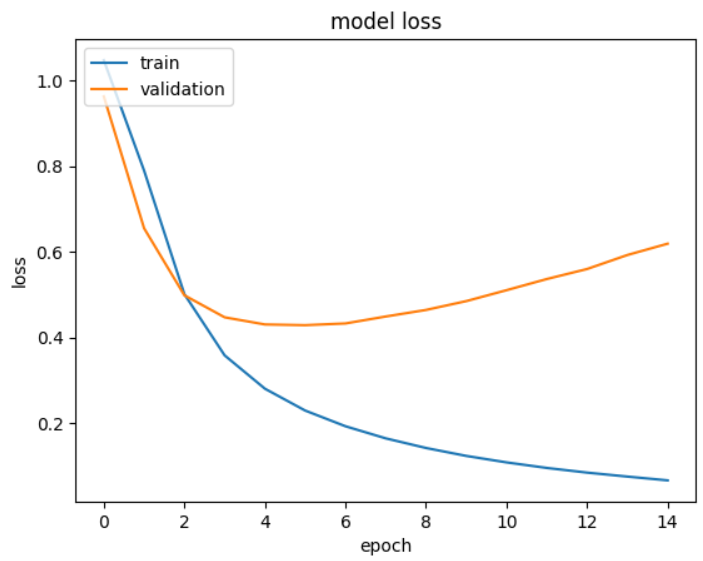
\includegraphics[width=0.5\linewidth]{loss.png}
    \caption{Graph of model loss}
    \label{fig:enter-label}
\end{figure}

\begin{figure}[H]
    \centering
    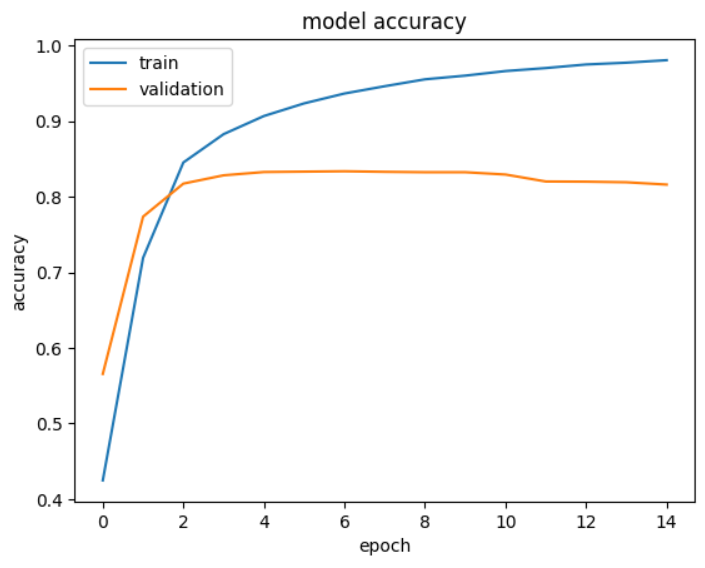
\includegraphics[width=0.5\linewidth]{accuracy.png}
    \caption{Graph of model accuracy}
    \label{fig:enter-label}
\end{figure}

The model achieves a validation accuracy of 82\% but as we can see from the graph the validation loss starts to go up after 5 epochs, which indicates that model is overfitting, As a solutiion L2 Regularization could be used. \\ 

After running the model for 100 epochs with L2 Regularization coefficient of 0.01, the final obtained results are: 

\begin{figure}[H]
    \centering
    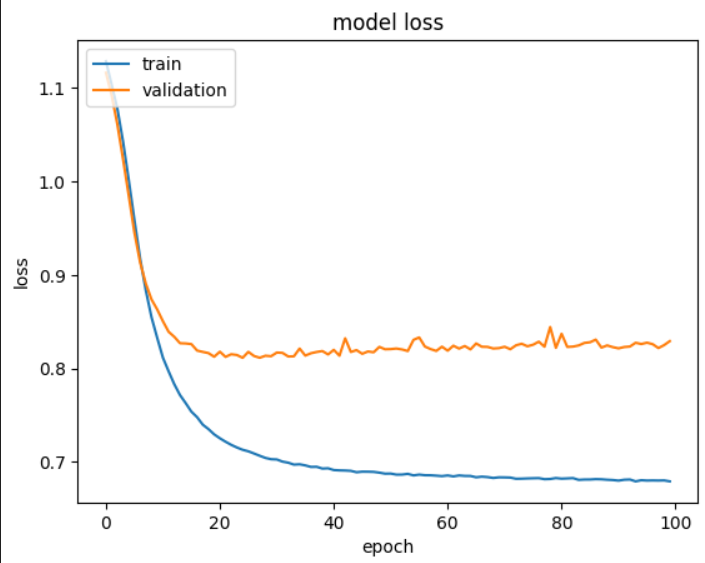
\includegraphics[width=0.5\linewidth]{l2 loss.png}
    \caption{Loss after adding L2 Regularization}
    \label{fig:enter-label}
\end{figure}

\begin{figure}[H]
    \centering
    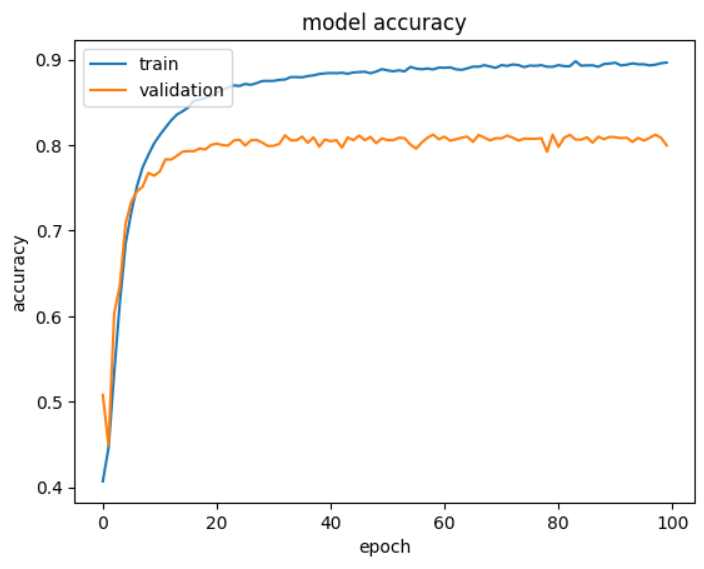
\includegraphics[width=0.5\linewidth]{l2 accuracy.png}
    \caption{Accuracy after adding L2 Regularization}
    \label{fig:enter-label}
\end{figure}

\subsection{Metrics results:}

\begin{itemize}
  \item Validation accuracy: 0.8123084902763367
  \item Validation precision: 0.8542508161067963
  \item Validation recall: 0.7597037553787231
  \item Validation F1 score: 0.8042079549144123 \\
\end{itemize}

As we can see we have improved all metrics except for recall.

\end{document}